\label{chap:discussion}

\epigraph{Our imagination is the only limit to what we can hope to have in the future.}{\textit{Charles F. Kettering \\ American inventor, engineer and businessman }}

\section{Conclusions}

\section{Future work}

This study deals only with one subsystem of the LSP station at HiLASE, namely, creating a robotic arm controller program for a three-dimensional part and it gives a peek into the future direction of the PhD thesis. The LSP station consists of several subsystems. Figure \ref{fig:subsystems} displays a mind map of the various LSP station subsystems. Each subsystem takes care of a certain aspect of the LSP process. Unfortunately, each subsystem has its unique control software. The ultimate goal of the PhD thesis is to create a  Supervisory Control And Data Acquisition (SCADA) control system to unify the fragmented subsystem's control software. 

\begin{figure}[h]
    \centering
    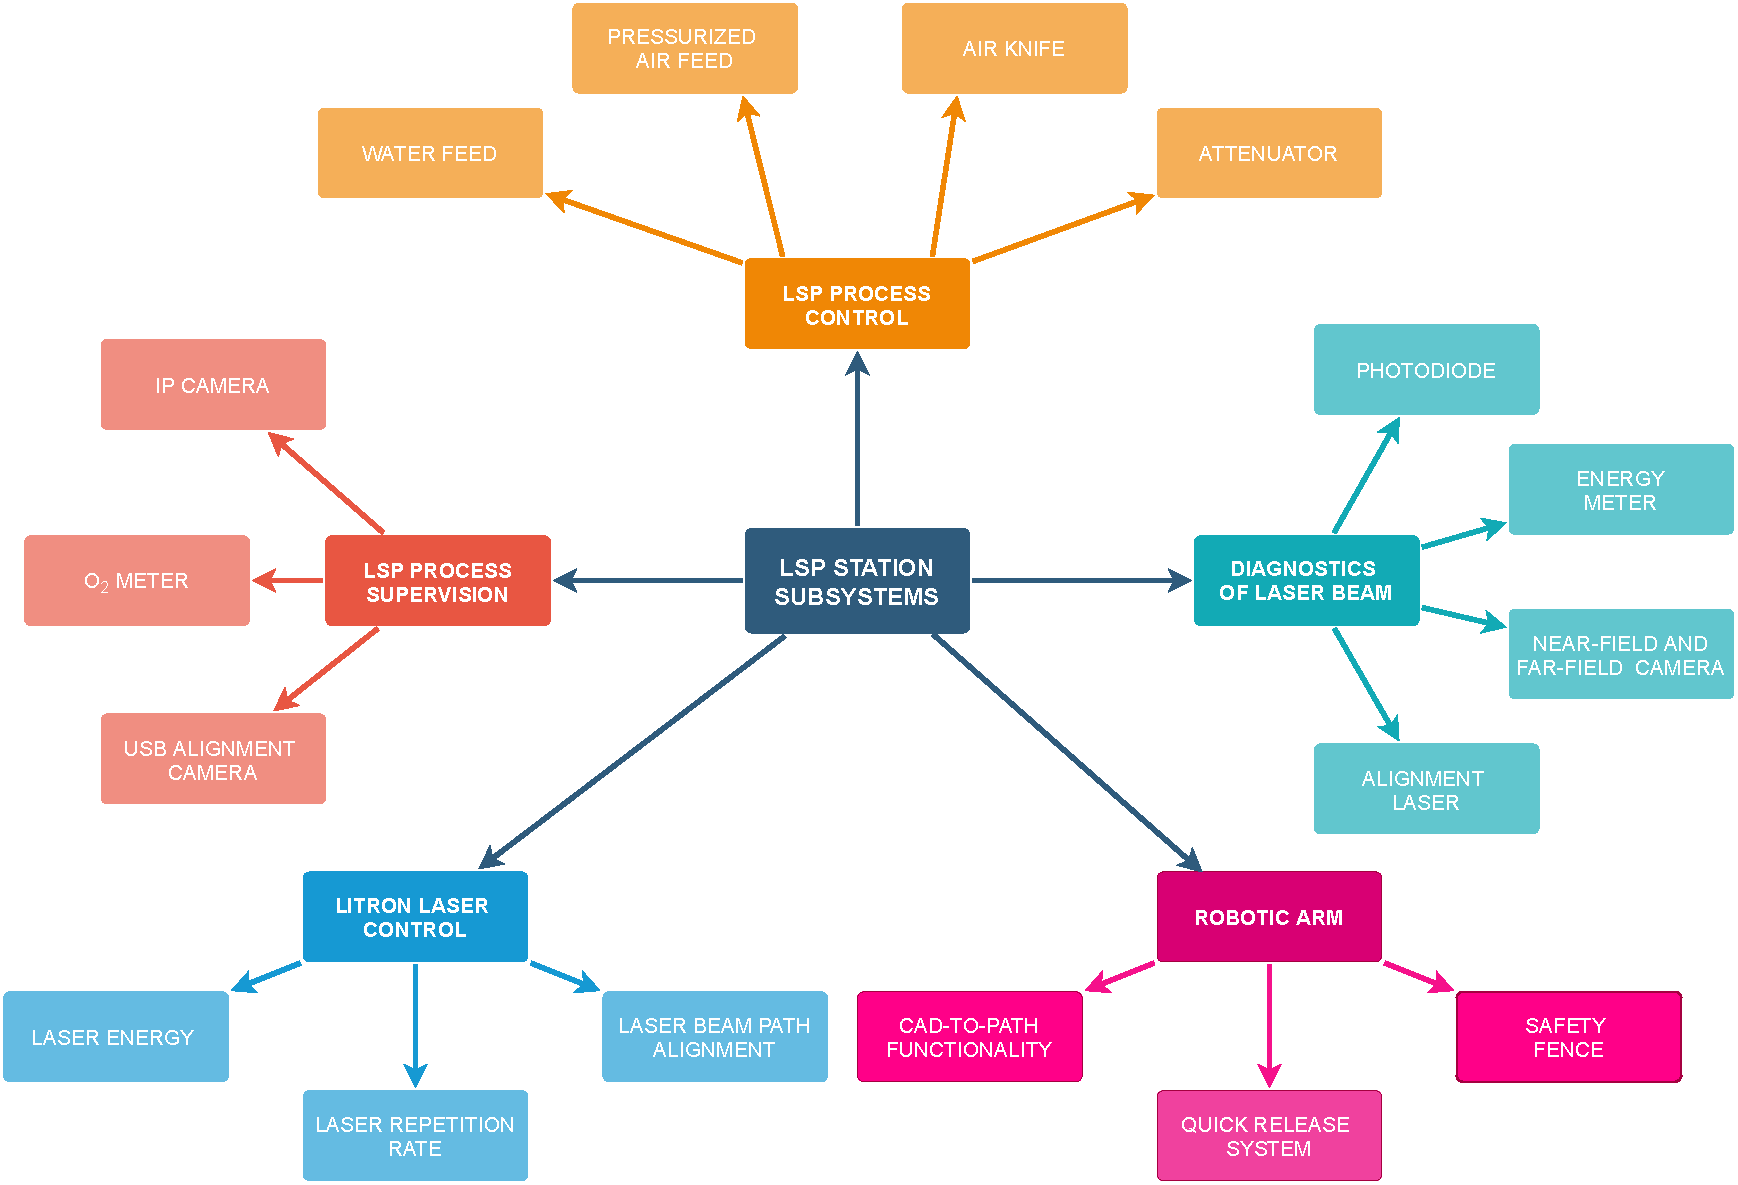
\includegraphics[width=1.0\linewidth]{img/lsp_subsystems.pdf}
    \caption{Mind map of the various LSP station subsystems}
    \label{fig:subsystems}
\end{figure}


The subsystems will be integrated using LabVIEW. LabVIEW (Laboratory Virtual Instrument Engineering Workbench) will be the development environment used in the PhD thesis. LabVIEW uses a graphical notation to create applications instead of lines of text. LabVIEW programs are called Virtual Instruments (VIs). LabVIEW is used for data acquisition, signal processing, and hardware control.

A LabVIEW program consists of the front panel window and the block diagram window. The front panel window contains controls and indicators (i.e., inputs and outputs). The block diagram window contains terminals corresponding to front panel controls and indicators, as well as constants, functions, structures, and wires that connect data from one object to another \cite{bress_2013}.


\subsection{Robotic arm Human-Machine Interface for LSP applications}


